\include{lecture_header}
\title{Environmental Fluid Dynamics: Lecture 2}
% colors
\definecolor{colororange}{HTML}{E65100} % orange
\definecolor{colordgray}{HTML}{795548} % dark gray for note
\definecolor{colorhgray}{HTML}{212121} % heavy dark gray for normal text
\definecolor{colorgreen}{HTML}{009688} % green
\definecolor{colorwhite}{HTML}{FFFFFF} % background white
\definecolor{colorlgray}{HTML}{F5F3EE} % background light gray
\definecolor{colorblue}{HTML}{0277BB} % blue
\definecolor{colorred}{HTML}{CC0000} % red
\newcommand{\fontsizeone}{1.9em}

\newcommand{\framecard}[2][colorgreen]{
  {\setbeamercolor{background canvas}{bg=#1}
    \begin{frame}[plain]
    \vfill
    \begin{center}
     {#2}
    \end{center}
    \vfill
    \end{frame}
  }
}

\begin{document}

%----------------------------------------------------------------------------------------
%	TITLE & TOC SLIDES
%----------------------------------------------------------------------------------------

\begin{frame} 
  \titlepage
\end{frame}

%------------------------------------------------

\begin{frame}
\frametitle{Overview}
\tableofcontents
\end{frame}

%------------------------------------------------
\section{Near-Surface Radiation Balance} %
%------------------------------------------------
\framecard[colorred]{{\color{white}\Huge Near-Surface\\~\\Radiation Balance}}
%------------------------------------------------
\begin{frame}{Energy Balance over Salt Flats}
Utah's West Desert
\begin{figure}
	\includegraphics[width=\textwidth]{fig1.png}
	\newline \centering \tiny Hoch et al. (2014)
\end{figure}
\end{frame}

%------------------------------------------------
\begin{frame}{Energy Balance over Salt Flats: Total Balance}

\centering $R_N = H + LE + G + \eta$
\begin{figure}
	\includegraphics[width=\textwidth]{fig2.png}
	\newline \centering \tiny Higgins et al. (2012)
\end{figure}
\end{frame}

%------------------------------------------------
\begin{frame}{Energy Balance over Salt Flats: Residual Components}
\centering $R_N = H + LE + G + \boxed{\eta}$
\begin{figure}
	\includegraphics[width=\textwidth]{fig3.png}
	\centering \newline \tiny Higgins et al. (2012)
\end{figure}
$\eta(t) = S(t) + A(t) + W(t) + O_T(t)$
\end{frame}

%------------------------------------------------
\begin{frame}{Energy Balance over Salt Flats: Residual Components}
\centering $R_N = H + LE + G + \boxed{\eta}$
\begin{figure}
	\includegraphics[width=\textwidth]{fig3.png}
	\centering \newline \tiny Higgins et al. (2012)
\end{figure}
\begin{itemize}
	\item 59\% energy storage in the soil layer
	\item 30\% underestimates of the soil heat flux
	\item 1\% percent advection (not statistically significant)
\end{itemize}
\end{frame}

%------------------------------------------------
\section{Near-Surface Thermal Radiation} %
%------------------------------------------------
\framecard[colorred]{{\color{white}\Huge Near-Surface\\~\\Thermal Radiation}}
%------------------------------------------------
\begin{frame}{Near-Surface Thermal Radiation}

{\large \textbf{Radiation}}
\\\vspace{2pt}
\begin{fancydefs}
	Transfer of energy through rapid oscillation of electromagnetic fields
\end{fancydefs}
$$R_N = H + H_L + H_G + \Delta H_S$$
$$R_N = R_S(\downarrow) + R_S(\uparrow) + R_L(\downarrow) + R_L(\uparrow)$$
~\\~\\
See Chapter 3 in Arya
\end{frame}

%------------------------------------------------
\begin{frame}{Electromagnetic Spectrum}

\begin{figure}
	\includegraphics[width=0.8\textwidth]{fig4}
	\centering \tiny~\\figBergman et al. (2011)\\ \centering \small Range of interest for atmospheric radiative transfer\\solar $\sim$0.1-4 $\micro\metre$ (short wave), terrestrial $\sim$3-100 $\micro\metre$ (long wave)
\end{figure}

Absorption of Radiation
\begin{itemize}
	\item Orbital changes in electrons
	\item Molecular vibration changes
	\item Molecular rotation changes
\end{itemize}
\end{frame}

%------------------------------------------------
\begin{frame}{Radiation Characteristics}

\begin{figure}
	\includegraphics[width=0.8\textwidth]{fig5}
	\centering \tiny~\\Bergman et al. (2011)
\end{figure}

Complexity of radiation: up to \textbf{7 independent variables}
\begin{itemize}
	\item Space: $x$, $y$, $z$
	\item Time: $t$
	\item Direction: $\theta$, $\phi$
	\item Wavelength: $\lambda$
\end{itemize}
\end{frame}

%------------------------------------------------

\begin{frame}{EPFL Raman Lidar - Inelastic Scattering}
  
  \setlength{\fboxsep}{0pt}
\setlength{\fboxrule}{1pt}
\begin{columns}[T]
    \begin{column}{.55\textwidth}
    \begin{minipage}[c][.7\textheight][c]{\linewidth}
    \begin{itemize}
    	\item LIDAR - LIght Detection And Ranging
    	\item Measures water vapor mixing ratio during the day and night
    	\item Raw spatial and time resolutions of 1.25 m and 1 s respectively
    	\item Range 15–500 m
    	\item Solar blind (wavelengths shorter than 0.300 $\micro\metre$, where O$_3$ absorbs most radiation)
    	\item Raman Scattering (inelastic scattering) - Temp: rotational, MR: rotational/vibrational
    \end{itemize}
      \end{minipage}
    \end{column}
    \begin{column}{.55\textwidth}
      \includegraphics[width=\textwidth]{fig6.png}
      \centering \tiny~\\Froidevaux et al. (2013)
    \end{column}
  \end{columns}
  
\end{frame}

%------------------------------------------------

\begin{frame}{Raman Lidar - Seerdorf, CH}
 \begin{figure}
      \includegraphics[width=0.95\textwidth]{fig7.png}
      \centering \tiny~\\Froidevaux et al. (2013)
  \end{figure}
\end{frame}

%------------------------------------------------

\begin{frame}{Raman Lidar}
 \begin{figure}
      \includegraphics[width=\textwidth]{fig8.png}
      \centering \tiny~\\Froidevaux et al. (2013)
  \end{figure}
\end{frame}

%------------------------------------------------

\begin{frame}{Raman Lidar}
 \begin{figure}
      \includegraphics[width=\textwidth]{fig9.png}
      \centering \tiny~\\Froidevaux et al. (2013)
  \end{figure}
\end{frame}

%------------------------------------------------

\begin{frame}{Radiation Intensity - Spherical Coordinates  and Solid Angle}
Directional distribution of thermal radiation is described via solid angles. Solid angles are 2D angular spaces: 
\begin{columns}[T]
    \begin{column}{.6\textwidth}
    \begin{minipage}[c][.6\textheight][c]{\linewidth}
    \begin{itemize}
    \item 1D angular pace: $d\alpha = dl/r$\\
    radians [$\radian$]\\
	$dl$: infinitesimal length on a circle
	~\\~\\~\\~\\
	\item 2D angular space: $d\omega = dA_n/r^2$\\
	steradians $[\steradian]$\\
	$dA_n$: infinitesimal area on a sphere 
	\end{itemize}  
      \end{minipage}
    \end{column}
    \begin{column}{.45\textwidth}
    	\centering 
      \includegraphics[width=0.8\textwidth]{fig10a.png}\newline
      \includegraphics[width=0.8\textwidth]{fig10b.png}
      \centering \tiny~\\Bergen et al. (2011)
    \end{column}
  \end{columns} 
\end{frame}

%------------------------------------------------

\begin{frame}{Radiation Intensity - Spherical Coordinates  and Solid Angle}
\begin{figure}
	\includegraphics[width=\textwidth]{fig11.png}
\end{figure}
\end{frame}

%------------------------------------------------

\begin{frame}{Radiation Intensity}
Let’s consider an emitting point on a surface. This point can radiate into all directions contained within a hemisphere of radius r. 

\begin{columns}[T]
    \begin{column}{.5\textwidth}
    \begin{minipage}[c][.5\textheight][c]{\linewidth}
    \begin{itemize}
    \item $dA_n$: infinitesimal area on the hemisphere of radius $r$
	\item $\theta$: polar (zenith) angle
	\item $\phi$: azimuthal angle
	\item $d\omega$: infinitesimal solid angle 
	\end{itemize}  
      \end{minipage}
    \end{column}
    \begin{column}{.5\textwidth}
    \includegraphics[width=1\textwidth]{fig12.png}
	\centering \tiny~\\Bergen et al. (2011)
    \end{column}
  \end{columns} 

\end{frame}

%------------------------------------------------

\begin{frame}{Radiation Intensity - Solid Angle}
\begin{figure}
	\includegraphics[width=0.9\textwidth]{fig13.png}
\end{figure}
\begin{itemize}
	\item The infinitesimal area dAn is given by: 
	$$dA_n = r^2sin\theta d\theta d\phi$$
	\item The infinitesimal solid angle is given by:
	$$d\omega = dA_n/r^2 = \boxed{sin\theta d\theta d\phi}$$
\end{itemize}
\end{frame}

%------------------------------------------------

\begin{frame}{Spectral Radiance - Lambert's Law}
\begin{itemize}
	\item $L_{(r,s)}$: spectral power per unit area, per unit solid angle, per unit frequency at the point $r$ in the direction of the unit vector $s$
	\item \textbf{Lambert's Law}: the fractional decrease of spectral radiance is proportional to the mass of the absorbing or scattering material met by the beam along $ds$
\end{itemize}
\begin{figure}
	\includegraphics[width=0.4\textwidth]{fig14.png}
\end{figure}
\end{frame}

%------------------------------------------------

\begin{frame}{Radiation: Attenuation}
\begin{figure}
	\includegraphics[width=\textwidth]{fig15.png}
	\centering \tiny~\\Bailey et al. (2014)
\end{figure}
\end{frame}

%------------------------------------------------

\begin{frame}{Radiation: Scattering}
\begin{figure}
	\includegraphics[width=\textwidth]{fig16.png}
	\centering \tiny~\\Bailey et al. (2014)
\end{figure}
\end{frame}

%------------------------------------------------

\begin{frame}{Radiation: Emission}
\begin{figure}
	\includegraphics[width=\textwidth]{fig17.png}
	\centering \tiny~\\Bailey et al. (2014)
\end{figure}
\end{frame}

%------------------------------------------------

\begin{frame}{Shortwave and Longwave Radiation}
\begin{columns}[T]
\begin{column}{.5\textwidth}
    \begin{minipage}[c][\textheight][c]{\linewidth}
    \textbf{Wien's Displacement Law} - wavelength of maximum spectral emissive power
    $$\lambda_{\text{max}} = \frac{2898}{T_{\text{abs}}}$$
      \end{minipage}
    \end{column}
    \begin{column}{.5\textwidth}
    \includegraphics[width=1\textwidth]{fig18.png}\newline
      \includegraphics[width=0.9\textwidth]{fig19.png}
	\centering \tiny~\\Arya (2001)
    \end{column}
  \end{columns} 
\end{frame}

%------------------------------------------------

\begin{frame}{Average Global Radiation Balance}
\begin{figure}
	\includegraphics[width=\textwidth]{fig20.png}
	\centering \tiny~\\Radiation balance for the atmosphere
\end{figure}
\end{frame}

%------------------------------------------------

\begin{frame}{Radiative Properties of Surfaces}
\begin{columns}[T]
\begin{column}{.4\textwidth}
    \begin{minipage}[c][0.5\textheight][c]{\linewidth}
    \begin{align*}
    \alpha = \frac{R_S\uparrow}{R_S\downarrow} &= \int^{4\ \micro\metre}_{0.15\ \micro\metre} \alpha_\lambda d\lambda\\
    \epsilon &= \int^{100\ \micro\metre}_{3\ \micro\metre} \epsilon_\lambda d\lambda
    \end{align*}
    Albedo of wet grass is a few \% less than dry grass
      \end{minipage}
    \end{column}
    \begin{column}{.6\textwidth}
    \includegraphics[width=1\textwidth]{fig21.png}
	\centering \tiny~\\Arya (2001)
    \end{column}
  \end{columns} 
\end{frame}

%------------------------------------------------

\begin{frame}{Albedo Variability - Murray, Utah}
\begin{figure}
	\includegraphics[width=\textwidth]{fig22.png}
\end{figure}
\end{frame}

%------------------------------------------------

\begin{frame}{Surface Irradiance}
\begin{figure}
	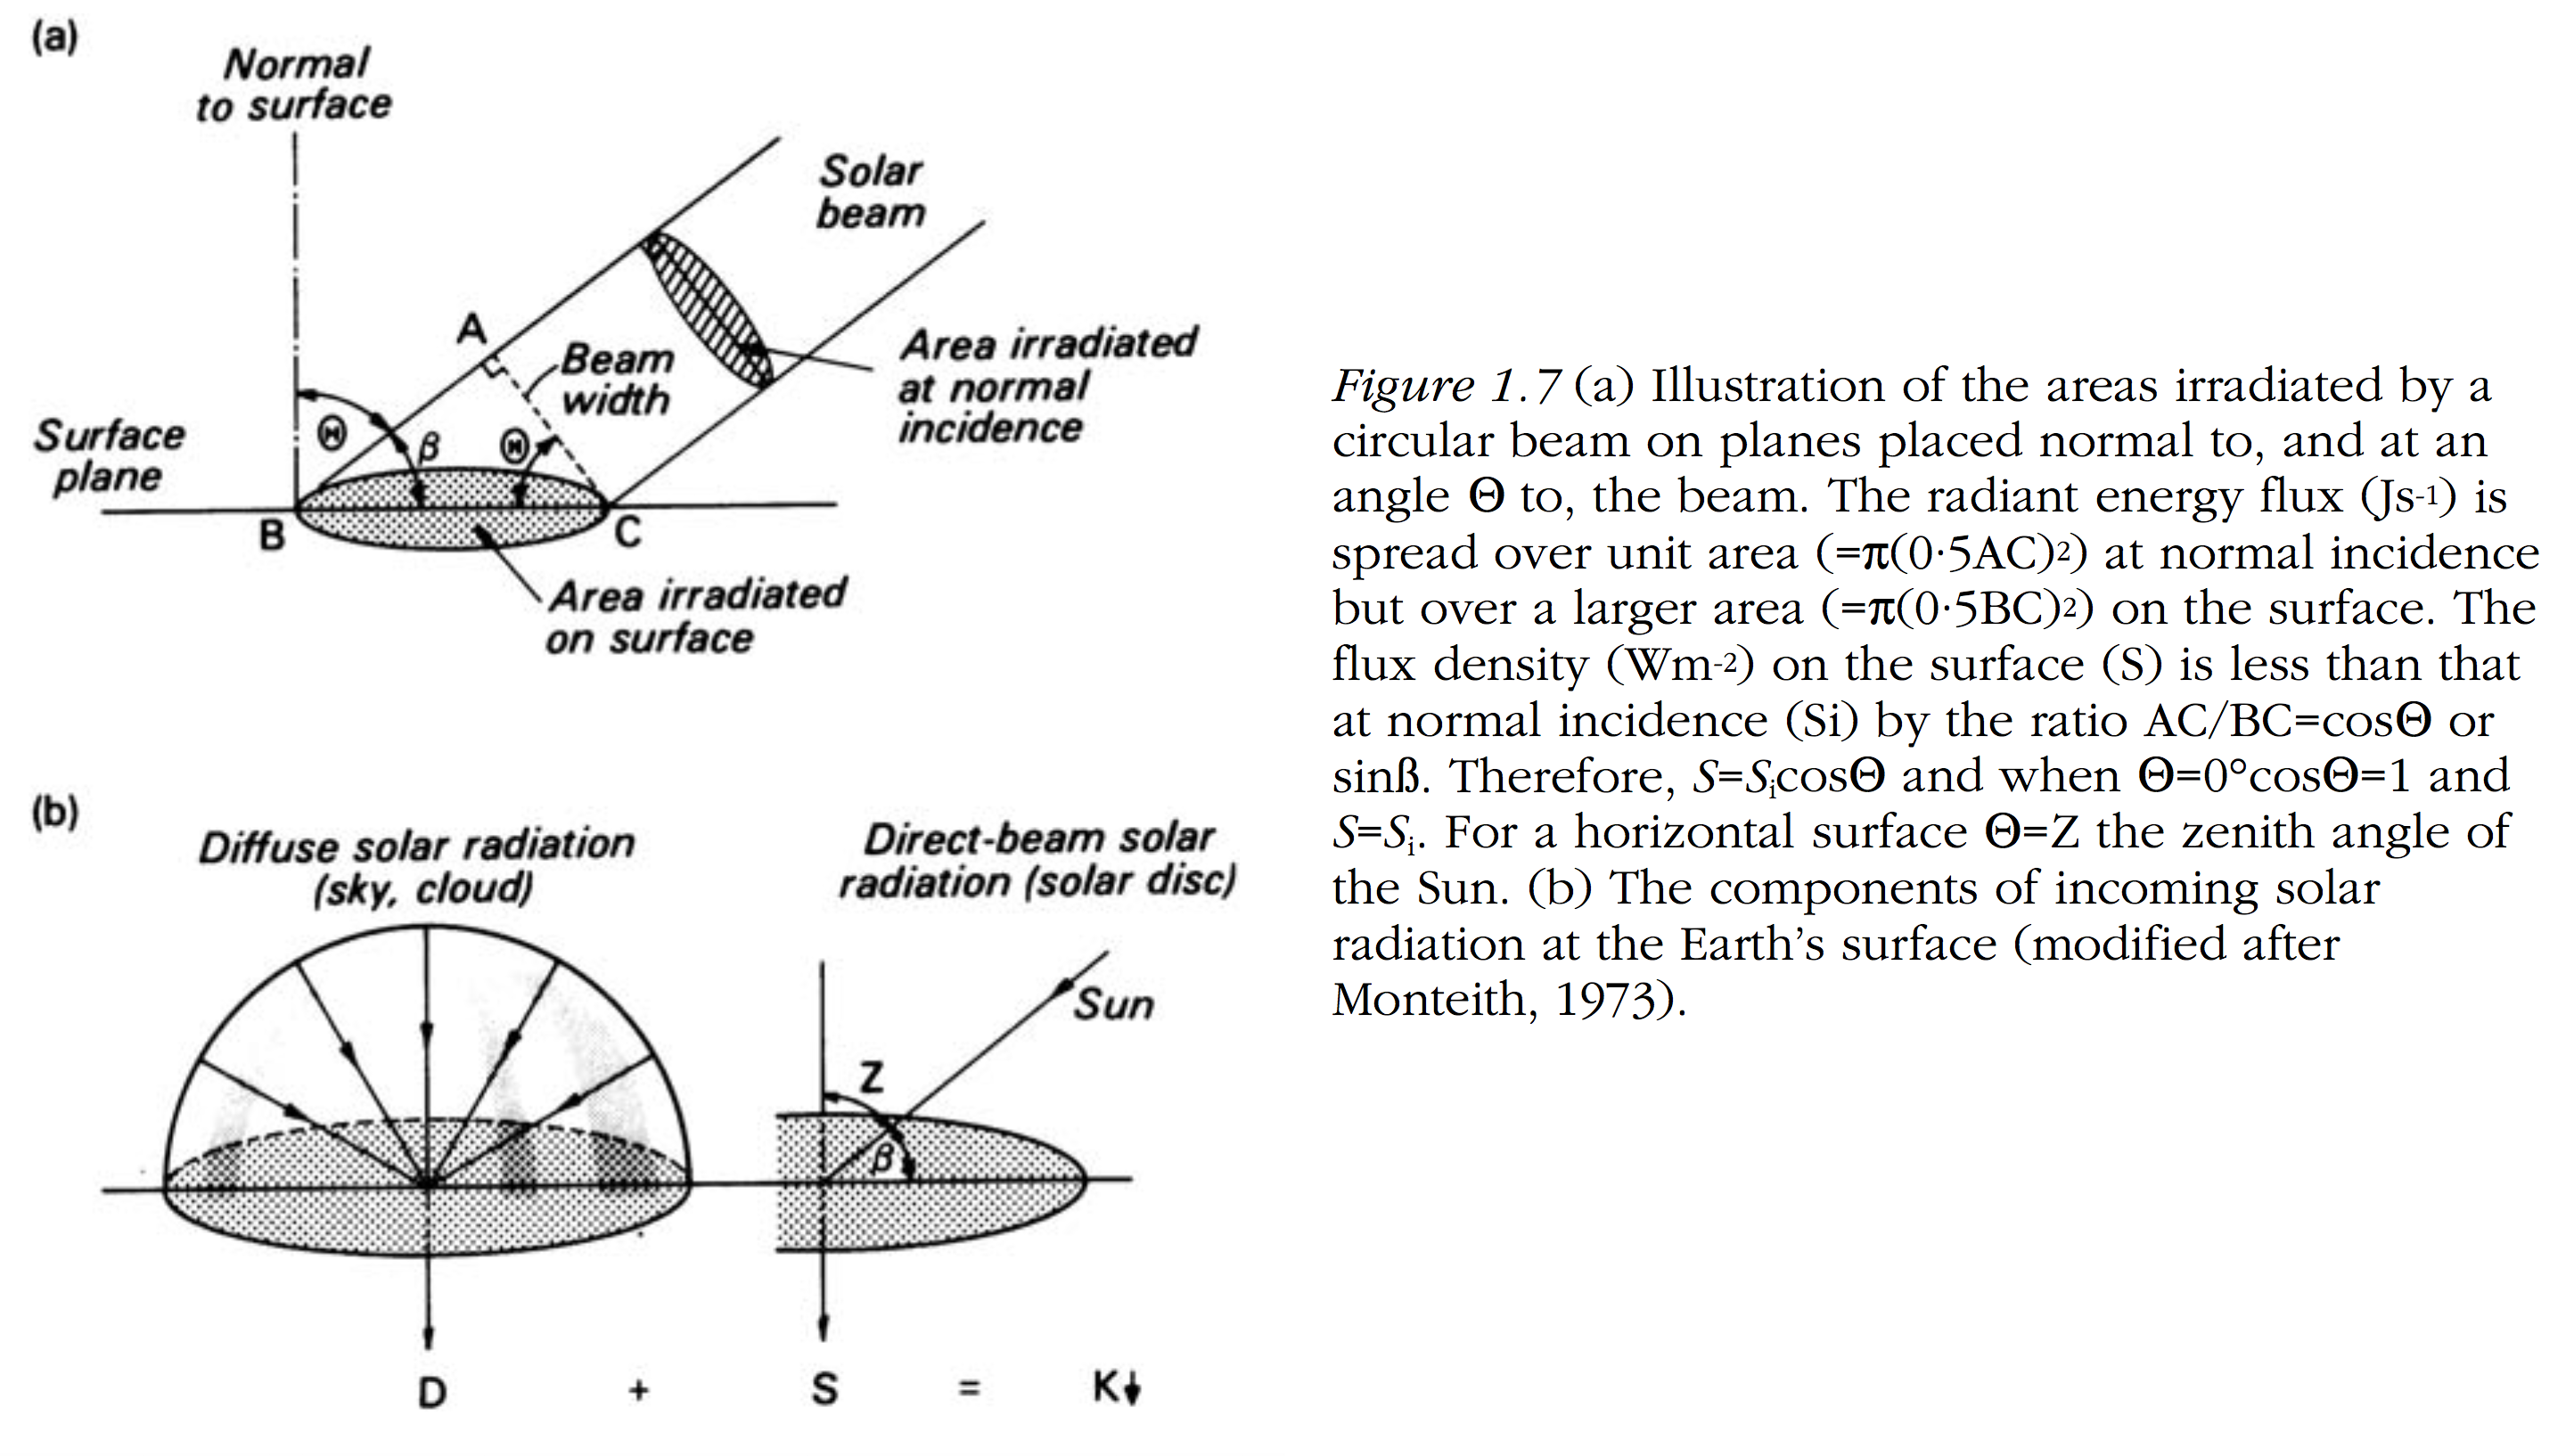
\includegraphics[width=0.9\textwidth]{fig23.png}
\end{figure}
\begin{itemize}
\small
	\item \textbf{Direct solar radiation}: portion of short-wave radiation received in a parallel beam ``directly'' from the sun
	\item \textbf{Diffuse solar radiation}: short-wave radiation reaching the Earth's surface after having been scattered from the direct beam by molecules or other agents in the atmosphere
\end{itemize}

\end{frame}

%------------------------------------------------

\begin{frame}{Surface Irradiance}
\begin{figure}
	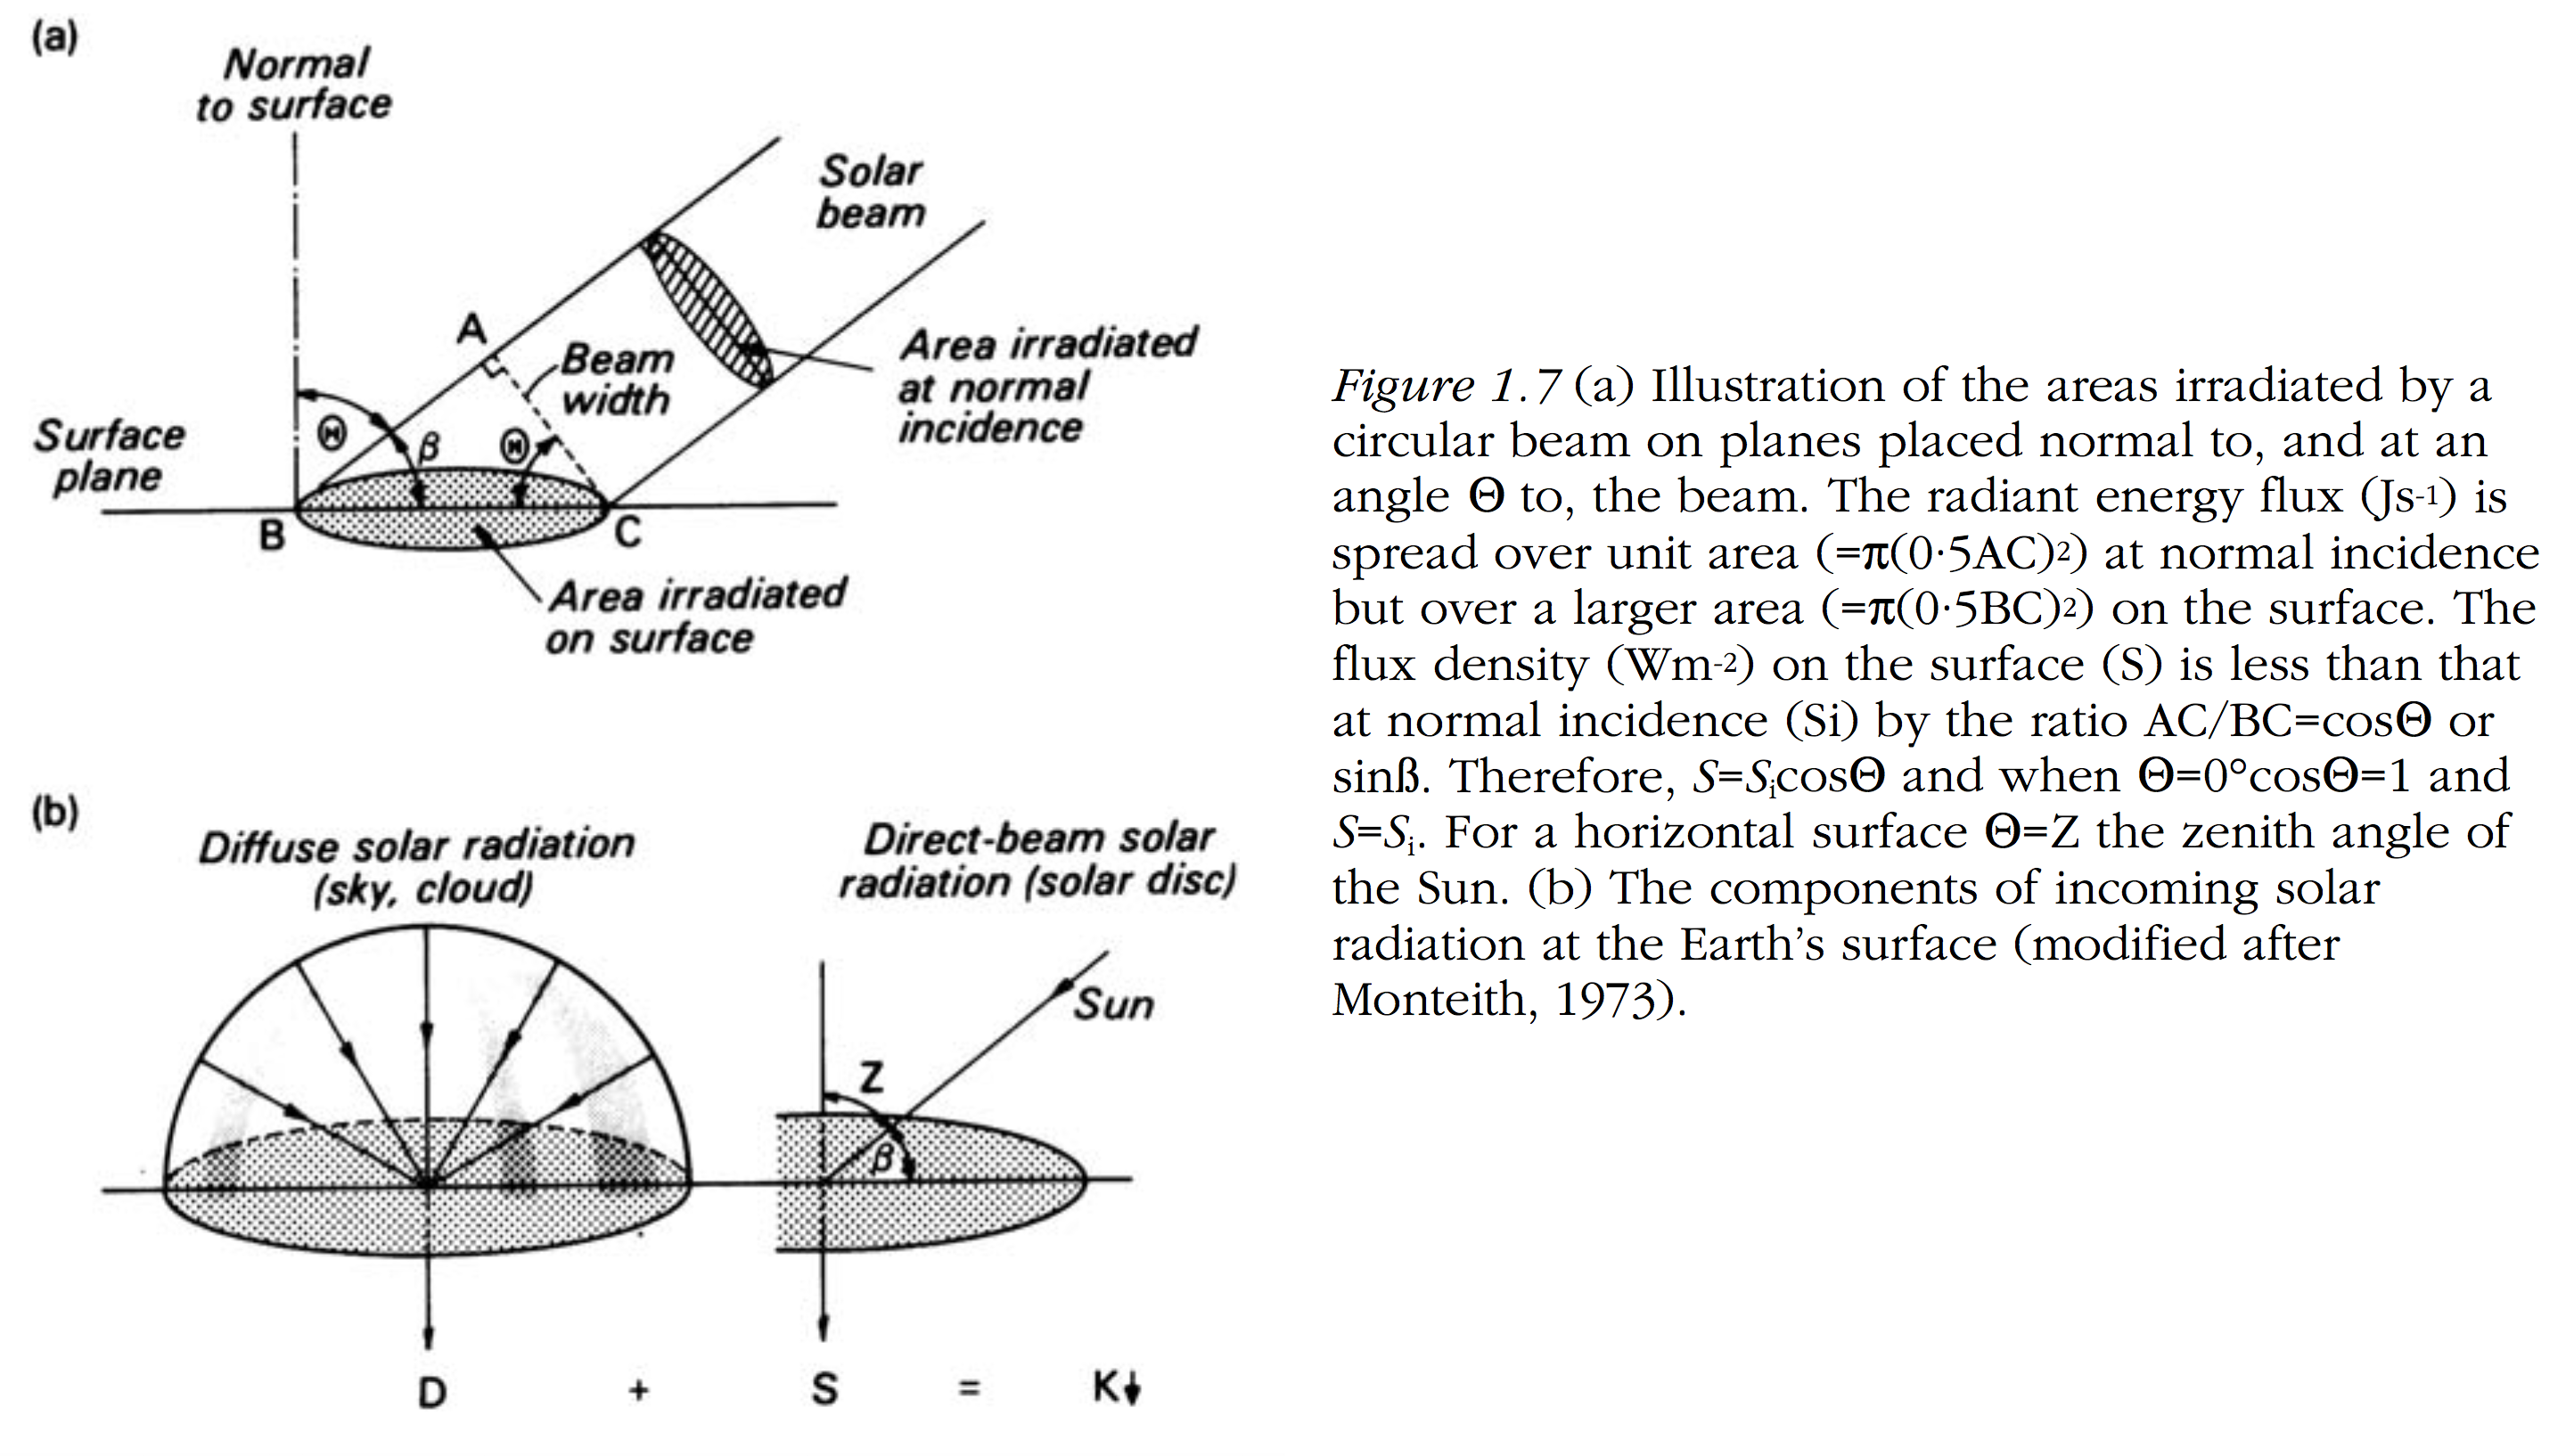
\includegraphics[width=0.9\textwidth]{fig23.png}
\end{figure}
\begin{itemize}
\small
	\item Global = direct solar radiation + diffuse solar radiation
	\item For clear conditions:
	\begin{itemize}
	\item diffuse: $\sim 10-20\%$
	\item direct: $\sim 80-90\%$
	\end{itemize}
\end{itemize}

\end{frame}

%------------------------------------------------

\begin{frame}{Direct/Diffuse Surface Irradiation}
\begin{figure}
	\includegraphics[width=0.7\textwidth]{fig25.png}
	\centering \tiny~\\Monteith and Unsworth (2013):
	\centering Cloudless day, Sutton Bonington, England
\end{figure}
\end{frame}

%------------------------------------------------

\begin{frame}{Solar ``Contant''}
\begin{figure}
	\includegraphics[width=\textwidth]{fig24.png}
	\centering \tiny~\\Monteith and Unsworth (2013)
\end{figure}
\end{frame}

%------------------------------------------------

\begin{frame}{Clear Atmospheric Flux Density of Solar Radiation }
\textbf{Irradiance Spectrum}
\begin{figure}
	\includegraphics[width=\textwidth]{fig26.png}
	\centering \tiny~\\Arya (2001)
\end{figure}
\end{frame}

%------------------------------------------------

\begin{frame}{Cloudless Absorption Spectra}
\begin{figure}
	\includegraphics[width=0.9\textwidth]{fig27.png}
	\centering \tiny~\\Arya (2001)
\end{figure}
\end{frame}

%------------------------------------------------

\begin{frame}{Radiation Balance (Clear Diffuse Component)}
K – Shortwave; L – Longwave; $\text{R}_n$ – Net Radiation
\begin{figure}
	\includegraphics[width=\textwidth]{fig28.png}
	\centering \tiny~\\Nadeau et al. (2012)
\end{figure}
\end{frame}

%------------------------------------------------

\begin{frame}{Radiation Balance}
K – Shortwave; L – Longwave
\begin{figure}
	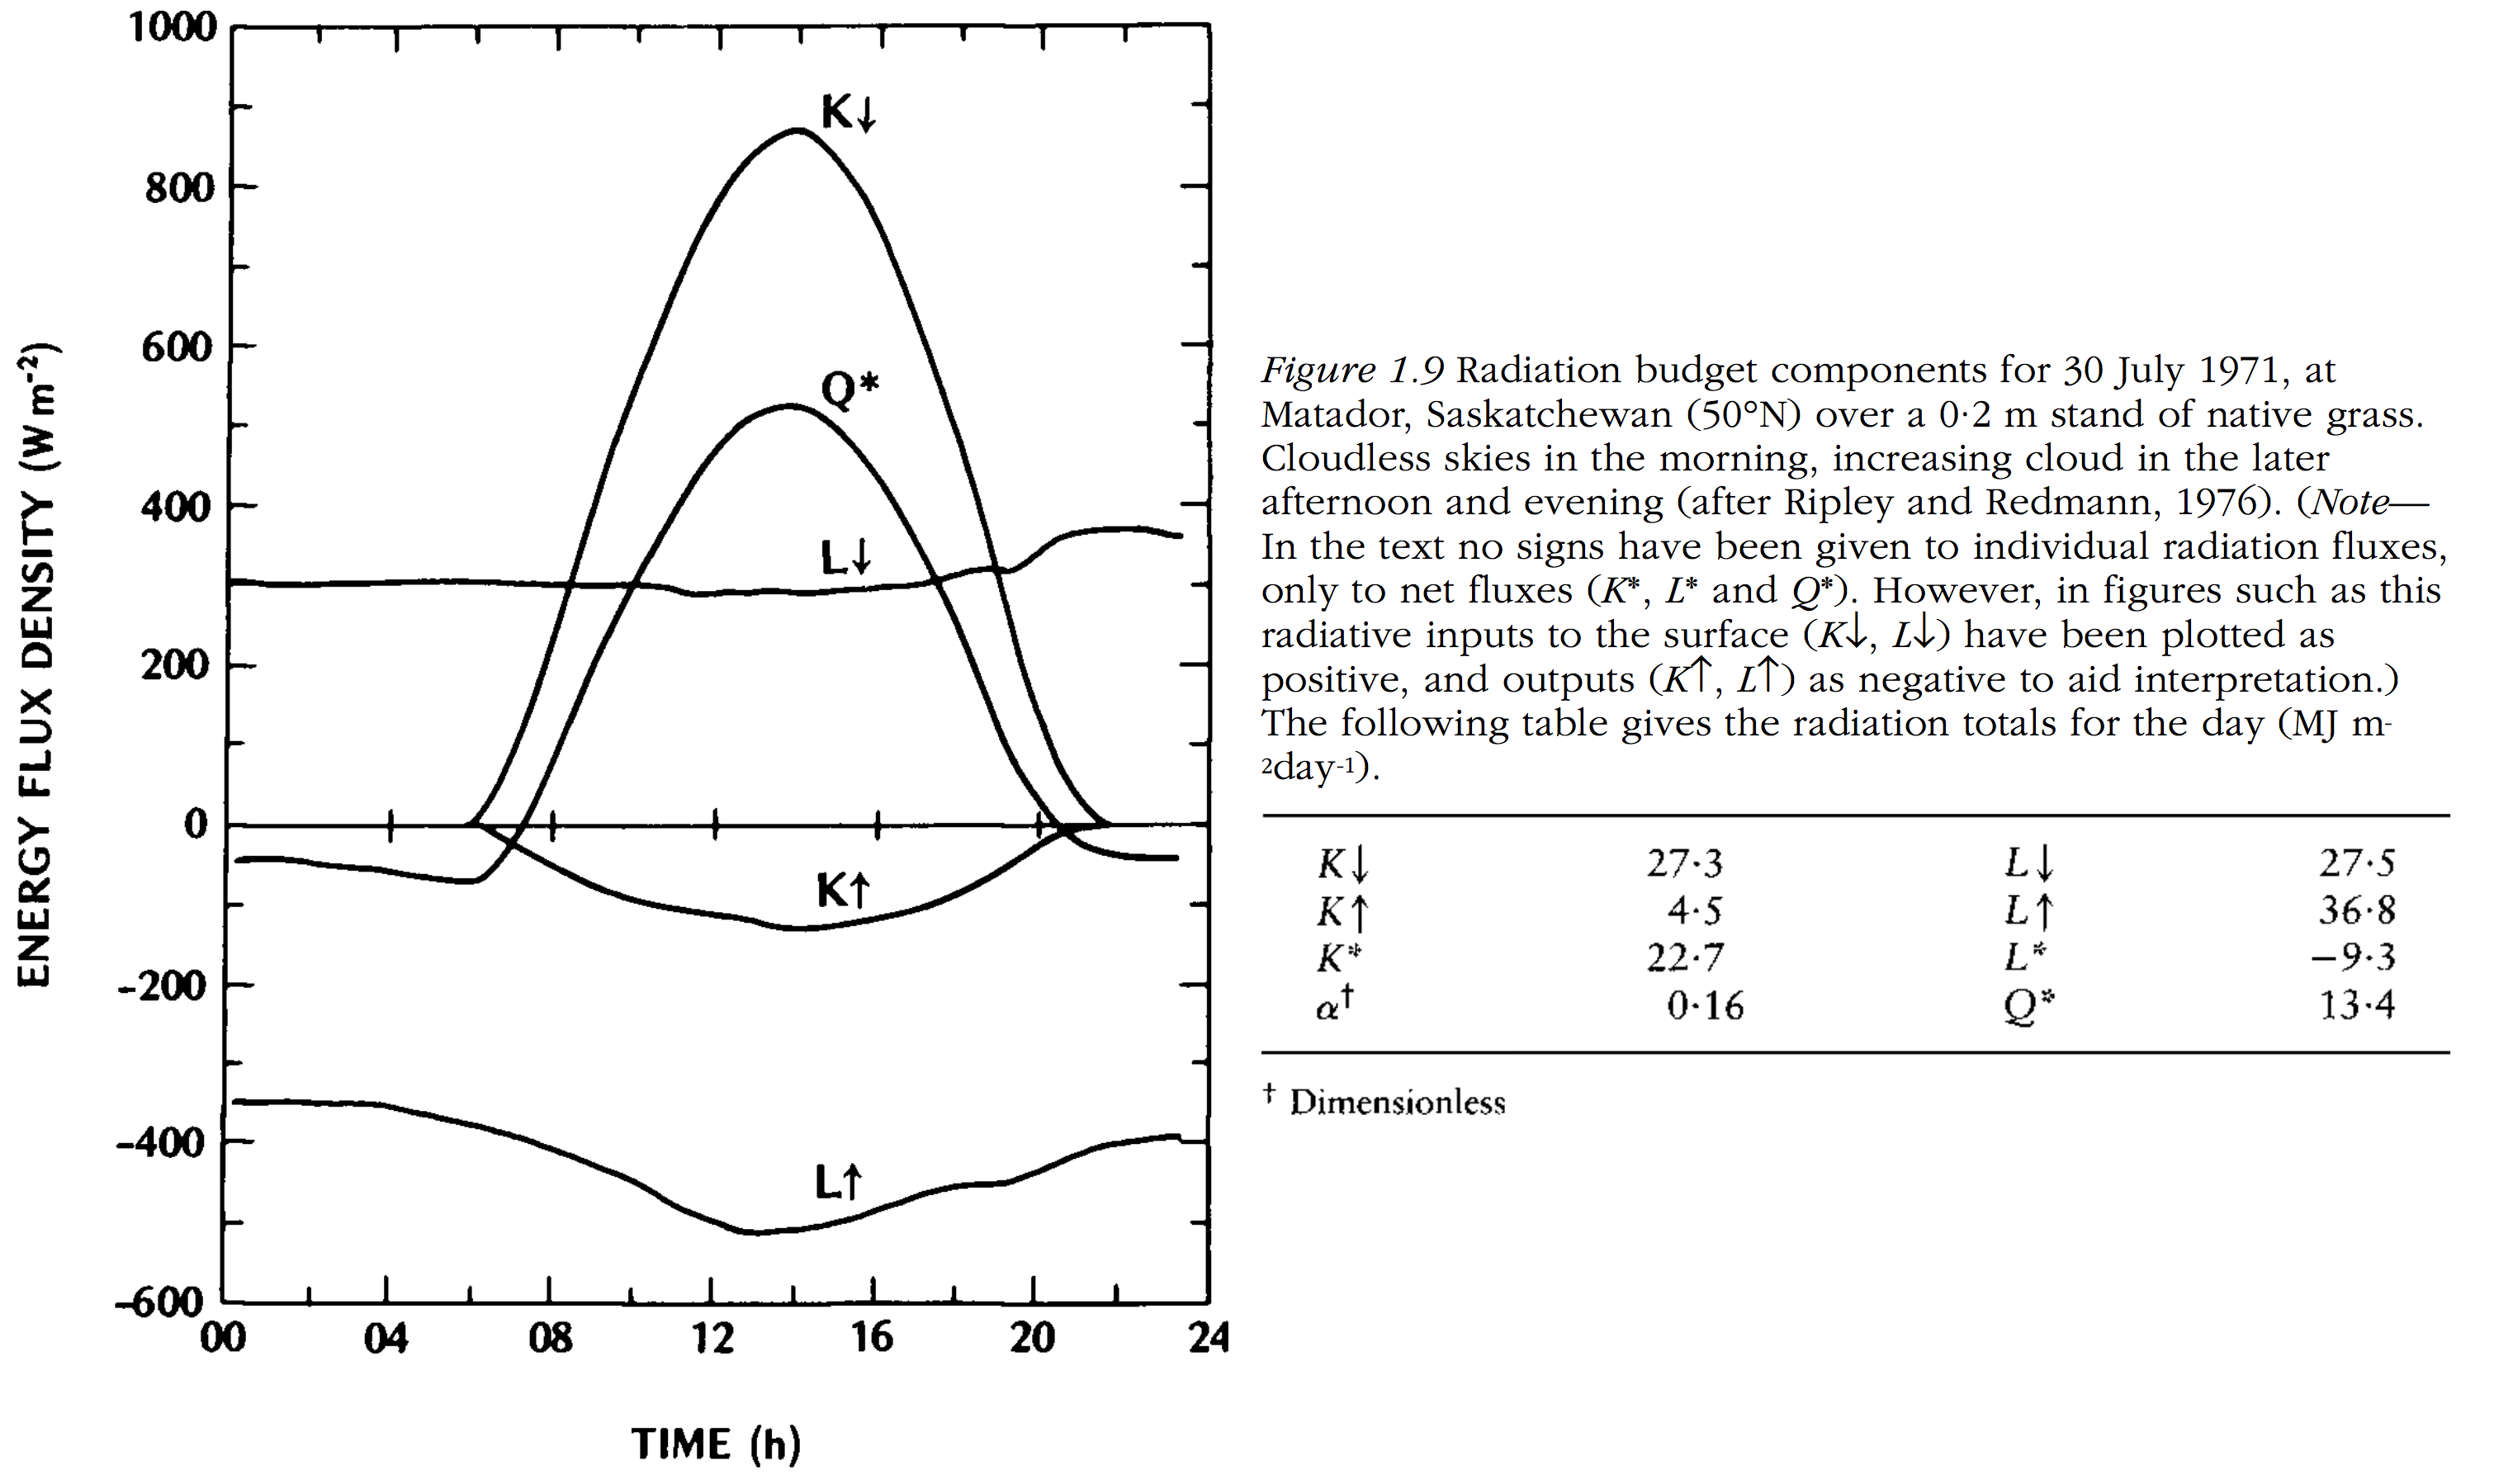
\includegraphics[width=\textwidth]{fig29.png}
	\centering \tiny~\\Oke (1987)
\end{figure}
\end{frame}

%------------------------------------------------

\begin{frame}{Slope Solar Beam Irradiance}
\begin{figure}
	\includegraphics[width=\textwidth]{fig30.png}
\end{figure}
\end{frame}

%------------------------------------------------

\begin{frame}{Slope Solar Beam Irradiance}
\begin{figure}
	\includegraphics[width=\textwidth]{fig31.png}
\end{figure}
\end{frame}

%------------------------------------------------

\begin{frame}{Slope Solar Beam Irradiance}
\begin{figure}
	\includegraphics[width=0.8\textwidth]{fig32.png}
	\centering \tiny~\\Oke (1987)
\end{figure}
$$\hat S = S_i cos \hat \Theta$$
\end{frame}

%------------------------------------------------

\begin{frame}{Slope Solar Beam Irradiance}
\begin{figure}
	\includegraphics[width=0.7\textwidth]{fig33.png}
	\centering \tiny~\\Oke (1987)
\end{figure}
\end{frame}

%------------------------------------------------

\begin{frame}{Direct Beam Solar Radiation on Sloped Surfaces}
\begin{figure}
	\includegraphics[width=0.48\textwidth]{fig34.png}
	\centering \tiny~\\Oke (1987)
\end{figure}
\end{frame}

%------------------------------------------------

\begin{frame}{Direct Beam Solar Radiation on Sloped Surfaces}
\begin{figure}
	\includegraphics[width=0.65\textwidth]{fig35.png}
	\centering \tiny~\\Oke (1987)
\end{figure}
\end{frame}

%------------------------------------------------

\end{document}

